\lhead{\emph{Methodology}}

\chapter{Methodology} \label{implementation}
The use of gaps in \acrshort{lipp} trees is crucial for supporting subsequent key insertions and reducing the number of shifts and conflicts that occur during insertion operations. However, the handling of conflicts in \acrshort{lipp}  trees differs from other tree structures like \acrshort{alex}. While \acrshort{alex} uses the shifting method to handle conflicts, \acrshort{lipp}  trees create a new child node. This method guarantees that items remain sorted, but it introduces extra computation cost during insertion operations.

The objective of this study is to explore methods of optimizing mutable tree-based \learnindex by strategically creating gaps for future insertions to minimize conflicts. This approach differs from \acrshort{fmcd} \cite{LIPP}. The study investigates two initial implementations: (1) Histogram, and (2) Partially sorted insertion strategy.

Our first implementation, Histogram, involves creating a histogram of the dataset to determine the frequency distribution of the keys. Based on this distribution, our algorithm leaves gaps in the appropriate places to accommodate future insertions, thereby reducing the number of conflicts that occur during insertion.

Our second implementation, Insert strategy partial sorted, focuses on identifying the most suitable location to insert a new key based on available space after the predicted position. The algorithm examines the dataset and creates a partially sorted list, which contains the keys in ascending order up to a certain point, and then the rest of the keys are left unsorted. This approach allows for more efficient insertion by taking advantage of the sorted section of the list while still leaving room for new keys to be inserted without causing conflicts.

\section{Histogram}
Histogram is a sequence of bin and bin is a partition of a range of keys which represents the distribution of the keys in the node.
Maintaining a histogram in each node of the \acrshort{lipp} tree structure is a powerful method for optimizing the placement of gaps in the array. \acrshort{lipp} triggers rebuilding of tree nodes when the node's depth is two times. We use histogram to approximate the distribution of the items in the gapped array and insert gaps based on the distribution and then train the model based on the the keys' position. 

However, the success of this method depends on selecting an appropriate bin size for the histogram. The challenge is to strike a balance between the overfitting and underfitting of the data in the histogram. Overfitting occurs when the bin size is too small, which leads to too many bins and lack of generalization to unseen data. Underfitting occurs when the bin size is too large, which leads to fewer bins and a loss of detail in the data.

There are several methods for selecting an appropriate bin size for the histogram, including the \acrfull{fdrule} and Sturges' rule \cite{sahann2021histogram}. For our histogram algorithm, we use Freedman-Diaconis rule to attain the bin width for the histogram.
Each nodes has its own bin width to reflect on the data in its gapped array and its subtree. 

The Freedman-Diaconis rule is a method for determining an appropriate bin width for creating a histogram. Histogram is useful for visualizing the distribution of a dataset. They work by dividing the range of data into a series of bins and counting the number of data points that fall into each bin. 

In addition, the bin width is an important parameter in constructing a histogram, as it determines the number of bins and the level of detail displayed in the frequencies of the keys. If the bin width is too small, the histogram may show too much detail and become difficult to read. If the bin width is too large, the histogram may lose important information and become overly simplified.

\begin{equation}\label{eq:IQR}
    IQR = Q_3 - Q_1
\end{equation}


The Freedman-Diaconis rule aims to find an appropriate bin width that balances these trade-offs. It is based on the \acrfull{iqr} of the data (Equation \ref{eq:IQR}), which is a measure of the spread of the data that is less sensitive to outliers than the range or standard deviation. The \acrshort{iqr} is calculated by subtracting the value at the 25th percentile $(Q_1)$ from the value at the 75th percentile $(Q_3)$. It represents the range of the middle 50\% of the data.

\begin{equation}\label{eq:FreedmanDiaconis}
    Bin Width = \frac{c\times IQR}{\sqrt[3]{n}}
\end{equation}

The rule then calculates an "optimal" bin width as the product of a constant factor (usually set to 1.0) and the \acrshort{iqr}, divided by the cube root of the number of data points (Equation \ref{eq:FreedmanDiaconis}). This formula scales the bin width with the sample size, so that the bin size becomes smaller as the sample size increases. The cube root is used to find a balance between having too few bins and too many bins.

The Freedman-Diaconis rule is particularly useful for datasets that have a skewed or multimodal distribution. These types of datasets can be difficult to visualize accurately with histograms using other methods. The rule adjusts the bin width to account for the spread of the data in the middle 50\% of the distribution, rather than just the range of the data. 

While our approach of using a histogram to analyze the distribution of collected data and selecting an optimal bin width has several advantages, it is important to note that there are certain limitations to this technique. One of the primary drawbacks is that it may not perform well on real-world datasets where the distribution of the data is random and does not follow a specific pattern or distribution.

In such cases, a histogram-based approach may not be as effective, as the data may be too complex and varied to be analyzed using a simple histogram. This may result in suboptimal bin width selection, which in turn can lead to less efficient adjustments to the \learnindex structure.



\section{Partial Sorted Array} \label{partialsorted}
To address extra computation issue, we propose another method that uses of a partially sorted array in \acrshort{lipp} trees \cite{partialMonotonic}. A partially sorted array allows the algorithm to continue the search for the correct position of a new key forward until it reaches a specified limit. For example, when inserting a key $1.2$ into the gapped array $[1,2, GAP,3]$, the algorithm would ideally insert the key between one and two to maintain sorting. However, with partial sorting, the algorithm continues searching until it hits the limit $key+\epsilon$, where $\epsilon$ is a pre-defined limit. In this case, the algorithm scans forward until it reaches the number that is not more than three.

Partial sorting reduces the number of conflicts during insertion operations, but it does not completely eliminate them. Partially sorted arrays delay conflicts for future insertions, meaning conflicts will eventually occur when the available space runs out. For example, if the array is $[1,2,1.2,3,4, GAP]$ and the key $2.4$ is inserted, the algorithm must search beyond $4$ to find the gap. To address this issue, a limit $\epsilon$ is introduced to specify the amount of space to scan after the actual position where the insertion is intended. If space is exhausted after $key + \epsilon$, a new child node is created to hold the remaining keys.

When performing a range query on a partially sorted array, the algorithm does not scan from the beginning to the end of the range. Instead, it scans forward until it reaches the limit specified during the insertion operation to ensure the correctness of the range query. The use of partially sorted arrays in \acrshort{lipp} trees aims to amortize the cost of slow insertion, where the algorithm has to scan until it reaches the $key+\epsilon$ limit, with fast insertion where there is still space available.




% \begin{figure}
%     \centering
%     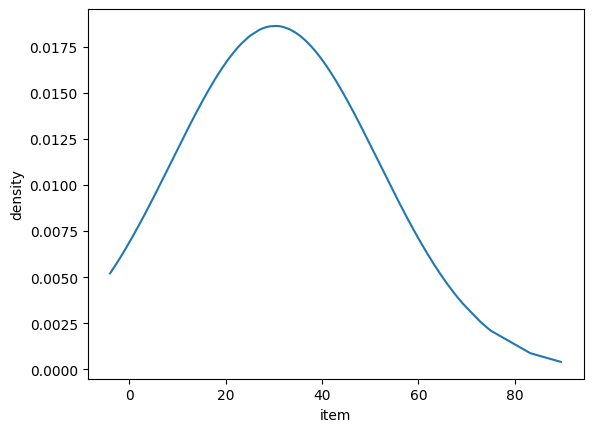
\includegraphics[width=80mm,scale=1]{Figures/normaldist.png}
%     \caption{
%         Normal distribution of Synthetic dataset
%     }
%     \label{fig:NormalDist}
% \end{figure}

% \subsubsection{Histogram}
% \begin{figure}
%     \centering
%     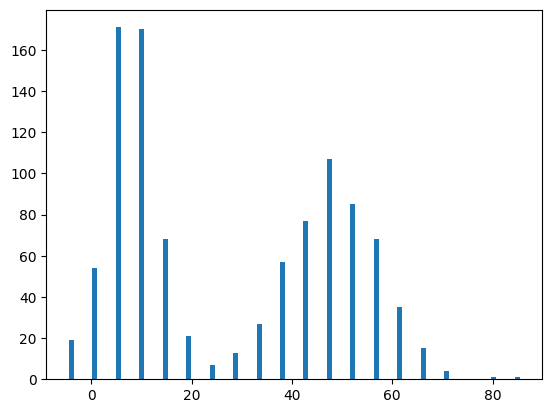
\includegraphics[width=80mm,scale=1]{Figures/histogram.png}
%     \caption{
%         Histogram of Synthetic data
%     }
%     \label{fig:Histogram}
% \end{figure}

% \subsubsection{Insert strategy Partial Sorted}





